\documentclass[a4paper,12pt]{article}
\usepackage[ukrainian,english]{babel}
\usepackage{ucs}
\usepackage[utf8]{inputenc}
\usepackage[T2A]{fontenc}
\usepackage{amsmath}
\usepackage{amsfonts}
\usepackage{graphicx}
\usepackage{tabto}
\usepackage[left=20mm, top=20mm, right=20mm, bottom=20mm, nohead, nofoot]{geometry}
\usepackage{hyperref}
\usepackage[paper=portrait,pagesize]{typearea}% for landscape orientation
\usepackage{changepage}% for adjustwidth
\usepackage{subcaption}% for subfig

\usepackage{tikz}
\newcommand\round[2]{\par
    \noindent\begin{tikzpicture}%
        \node[draw = #1, fill = #1, rectangle, rounded corners, 
              minimum size = 5.5mm, text = black, text width = 15cm, font = \ttfamily](char){#2};
    \end{tikzpicture}\par%
}%

\addto\captionsenglish{\renewcommand{\figurename}{Рис.}}
\addto\captionsenglish{\renewcommand{\tablename}{Таблиця}}

\begin{document}

\begin{titlepage}
		\begin{center}
		$\newline$
		\vspace{3.3cm}
		
		{\LARGE\textbf{Лабораторна робота №2\\з предмету\\Теоретико числові алгоритми}}
		\vspace{10cm}
		\begin{flushright}
			\textbf{Роботу виконала:}\\Бекешева Анастасія\\3-го курсу\\групи ФІ-12
		\end{flushright}
		\vspace{2cm}
		\begin{flushright}
			\textbf{Приймав:}\\Якимчук Олексій
		\end{flushright}
	\end{center}
\end{titlepage}
\newpage
\section{Мета.}
Ознайомлення з алгоритмом дискретного логарифмування Сiльвера-Полiга-Геллмана. Практична
реалiзацiя цього алгоритму. Пошук переваг, недолiкiв та особливостей застосування даного алгоритму
дискретного логарифмування. Практична оцiнка складностi роботи алгоритму.
\section{Постановка задачі.}
Написати програму, що реалiзовує алгоритм Сiльвера-Полiга-Геллмана для груп типу $\mathbb{Z}_p*$.
\section{Хід роботи.}
\subsection{План.}
\begin{enumerate}
	\item Створення  \href{https://github.com/nastyabekesheva/NTA-labs/tree/main/lab-2}{github repo}. 
	\item Імплементація перебору.
	\item Імплементація СПГ.
	\item Підняття Docker.
\end{enumerate}
\subsection{Проблеми.}
В принципі проблем майже не було. Довго в голові крутила формулу з 5 пункту алгоритму, з іншим все ок.
\section{Результати.}
В таблиці \ref{fig:time} наведено заміри роботи алгоритму СПГ та перебору для чисел довжини від 3 до 15. Перебір перестав працювати на числах довжини 10. СПГ працювало на всіх, але для числ довжини від 8 для задачі 2 типу час був сильно більшим за час для задачі 1 типу. З рисунку \ref{fig:type1}, що СПГ сильно ефективніше перебору для задачі 1 типу, а з рисунку \ref{fig:type2} та \ref{fig:sph} видно, що СПГ справляється задачею типу 2 трошки гірше. З рисунку \ref{fig:bf} видно що перебір просто в якийсь момент  перестає працювати. 
\section{Висновки.}
СПГ загалом (очевидно) працює краще перебору. Перевірялись числа від 3 до 15, адже більші числа допоміжна програма просто не згенерувала, але вирогідно СПГ перестало працювати ефективно приблизно на числах довжини від 20.
\begin{figure}[!htb]
\minipage{0.45\textwidth}
  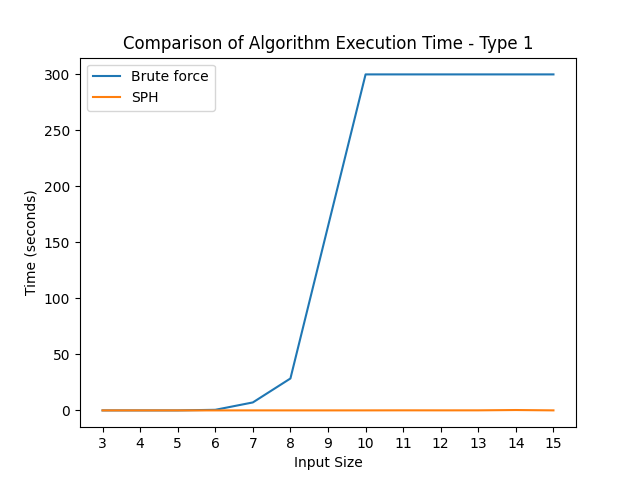
\includegraphics[width=\linewidth]{plot1.png}
  \caption{Задача типу 1}\label{fig:type1}
\endminipage\hfill
\minipage{0.45\textwidth}
  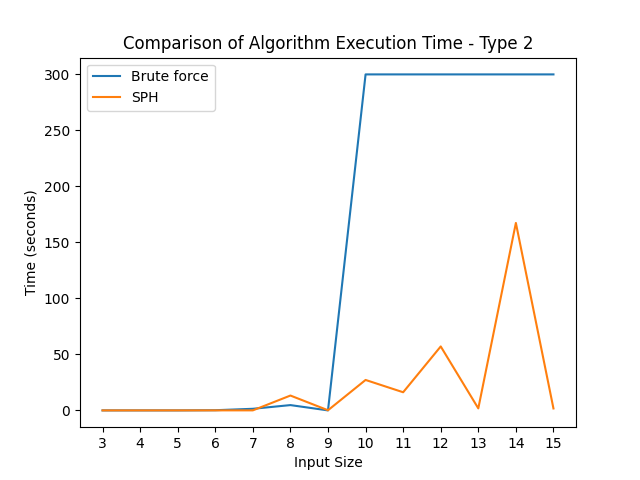
\includegraphics[width=\linewidth]{plot2.png}
  \caption{Задача типу 2}\label{fig:type2}
\endminipage\hfill
\end{figure}
\begin{figure}[!htb]
\minipage{0.45\textwidth}
  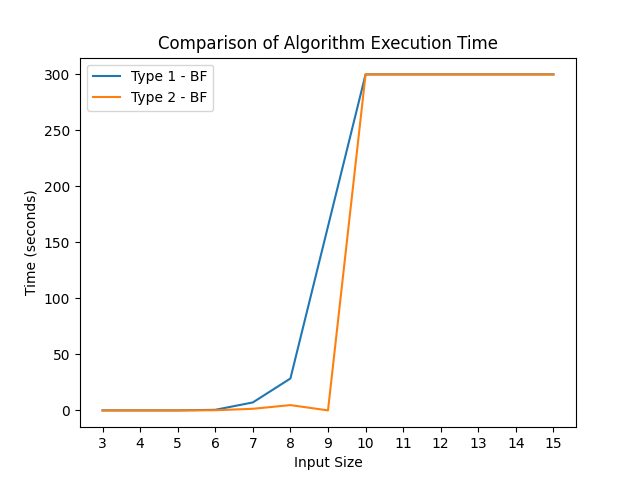
\includegraphics[width=\linewidth]{plot3.png}
  \caption{Перебір}\label{fig:bf}
\endminipage\hfill
\minipage{0.45\textwidth}
  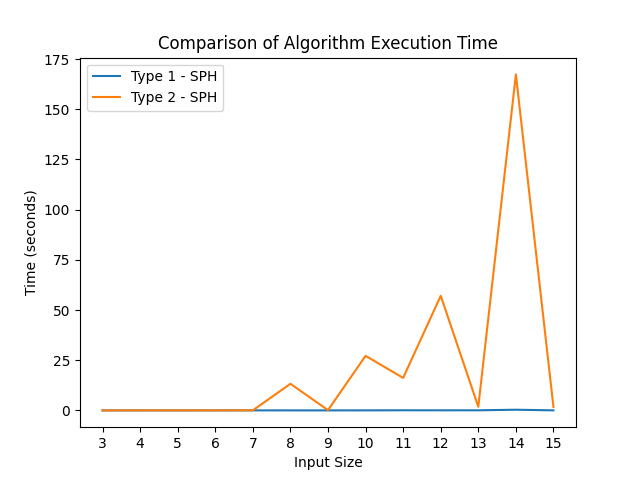
\includegraphics[width=\linewidth]{plot4.png}
  \caption{СПГ}\label{fig:sph}
\endminipage\hfill
\end{figure}
\begin{figure}[!htb]
\minipage{0.45\textwidth}
  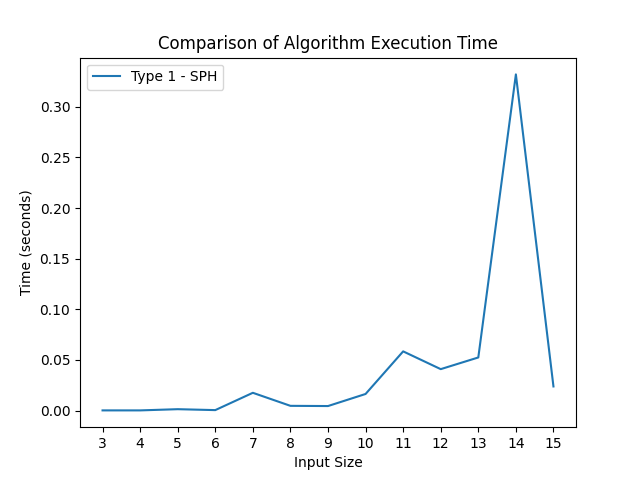
\includegraphics[width=\linewidth]{plot5.png}
  \caption{СПГ на задачі типу 1}\label{fig:sph1}
\endminipage\hfill
\minipage{0.45\textwidth}
  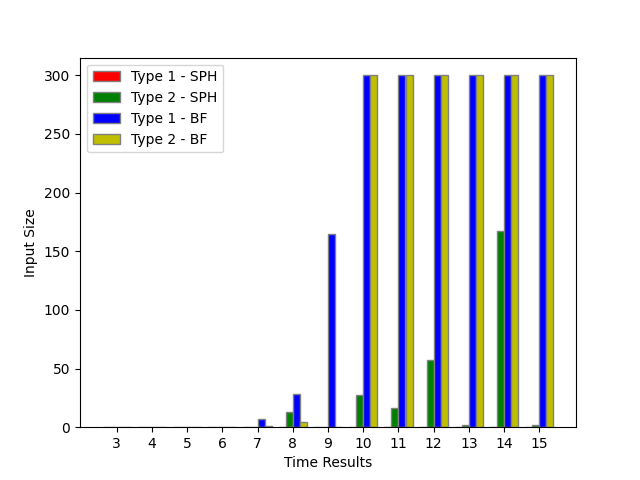
\includegraphics[width=\linewidth]{plot6.png}
  \caption{Bаr plot}\label{fig:Bаrplot}
\endminipage\hfill
\end{figure}\newpage 
\section{Docker.}
\round{gray!30}{docker run bekeshevaaa/nta-lab-2:0.1 a b p }
\newpage
	\KOMAoptions{paper=landscape,pagesize}
	\recalctypearea
\begin{table}[htp]
\begin{adjustwidth}{-5cm}{}
\begin{tabular}{||c|c|c|c|c|c|c||}\hline
Number of digits & $\alpha$ & $\beta$ & $p$ & $x$ & SPH time & BF time \\ \hline\hline
3 - Type 1 & 179 & 97 & 191 & 168 & 0.0002 & 0.0001 \\ \hline
3 - Type 2 & 2 & 437 & 491 & 226 & 0.0001 & 0.0001 \\ \hline
4 - Type 1 & 3086 & 2576 & 3617 & 1039 & 0.0002 & 0.0005 \\ \hline
4 - Type 2 & 3786 & 2919 & 4259 & 4085 & 0.0074 & 0.0021 \\ \hline
5 - Type 1 & 2417 & 11288 & 13627 & 1222 & 0.0014 & 0.0006 \\ \hline
5 - Type 2 & 606 & 19755 & 33773 & 9717 & 0.0108 & 0.0051 \\ \hline
6 - Type 1 & 69366 & 534740 & 889081 & 630451 & 0.0005 & 0.5202 \\ \hline
6 - Type 2 & 409634 & 294022 & 415607 & 221931 & 0.0275 & 0.1607 \\ \hline
7 - Type 1 & 3842476 & 6675652 & 8043979 & 7268042 & 0.0176 & 7.1154 \\ \hline
7 - Type 2 & 2742375 & 376513 & 4981313 & 1537567 & 0.0308 & 1.4344 \\ \hline
8 - Type 1 & 66830006 & 51535128 & 87321277 & 26090344 & 0.0047 & 28.4999 \\ \hline
8 - Type 2 & 3472738 & 5594295 & 14855123 & 4985397 & 13.2654 & 4.7348 \\ \hline
9 - Type 1 & 194476600 & 191132926 & 347205581 & 141181818 & 0.0045 & 164.3148 \\ \hline
9 - Type 2 & 197183379 & 197183379 & 256857593 & 128428797 & 0.1301 & 0.0000 \\ \hline
10 - Type 1 & 4551375215 & 1573551722 & 7870537313 & 7709472907 & 0.0164 & 300 \\ \hline
10 - Type 2 & 1372336390 & 1056512366 & 8080186871 & 826129382 & 27.1821 & 300 \\ \hline
11 - Type 1 & 14837213830 & 38662976351 & 44392159481 & 39230117359 & 0.0585 & 300 \\ \hline
11 - Type 2 & 17435029047 & 10429220418 & 31788610771 & 14754109763 & 16.2017 & 300 \\ \hline
12 - Type 1 & 543050355399 & 417773336744 & 740746544833 & 549000079782 & 0.0409 & 300 \\ \hline
12 - Type 2 & 258386314621 & 234508449353 & 948929348839 & 787937399626 & 57.1036 & 300 \\ \hline
13 - Type 1 & 3442360773292 & 4130940749100 & 5478710518453 & 3118837649776 & 0.0525 & 300 \\ \hline
13 - Type 2 & 7043450488041 & 3693873406607 & 9671170467619 & 6800381608693 & 1.7960 & 300 \\ \hline
14 - Type 1 & 26132929097130 & 18931503409489 & 90043656944741 & 24641734992724 & 0.3319 & 300 \\ \hline
14 - Type 2 & 2503177357728 & 5198261491908 & 22956856087093 & 6030786792897 & 167.3889 & 300 \\ \hline
15 - Type 1 & 145534237128898 & 59459578217324 & 234746379151573 & 191232194101023 & 0.0238 & 300 \\ \hline
15 - Type 2 & 72939729843574 & 106261771871845 & 290051083605971 & 32003267688517 & 1.7317 & 300\\ \hline
\end{tabular}
\end{adjustwidth}
\caption{Заміри часу}\label{fig:time}
\end{table}

\end{document}